%% LyX 2.0.8.1 created this file.  For more info, see http://www.lyx.org/.
%% Do not edit unless you really know what you are doing.
\documentclass[english]{article}
\usepackage[T1]{fontenc}
\usepackage[latin9]{inputenc}
\usepackage{array}
\usepackage{multirow}
\usepackage{amsmath}
\usepackage{graphicx}

\makeatletter

%%%%%%%%%%%%%%%%%%%%%%%%%%%%%% LyX specific LaTeX commands.
%% Because html converters don't know tabularnewline
\providecommand{\tabularnewline}{\\}

\makeatother

\usepackage{babel}
\begin{document}

\part*{Supplemental Methods}

The computations in this paper were run on the Odyssey cluster supported
by the FAS Division of Science, Research Computing Group at Harvard
University.


\section*{Transition Analysis}

A primary purpose of reconstructing GRNs is the understanding of the
biological mechanisms which characterize disease. Identifying differential
TF targeting may suggest a therapeutic target, uncover a disease substructure
or identify biomarkers for early detection. However, significant limitations
exist with respect to generating reliable context-specific GRNs. Substantial
advances have been made in this area with algorithms like SEREND and
PANDA, but these methods rely more heavily on the static sequence
motif data rather than gene expression data collected across groups,
such as in a case-control study. Both methods, along with BERE, use
gene expression data as a refinement of the more accurate motif priors.
It is therefore a side effect that any GRN inference method that relies
on motifs directly for edgeweight calculation will be susceptible
to having the bulk of its predictive power stripped when making comparisons
between networks. Consequently, it is of critical importance to choose
a network inference method that uses the context-specific data to
most accurately refine above what information is gleaned from our
static data.

The task of identifying meaningful network transitions then becomes
an evaluation of the relative refinement of edgeweights. Since the
majority of the predictive power for each edge is contained in the
motif contribution, we are left with relative edgeweight refinement
that have a low signal, high noise. In other words, we have a very
large number of individually unreliable edgeweights. In effort to
extract the maximum effect, we seek to combine the information contained
in each edge via a novel dimension reduction approach.

Consider two adjacency matrices, $\mathbf{A},\mathbf{B}$ representing
the two GRNs estimated from a case-control study. Each matrix has
dimensions $\left(p\times m\right)$ representing the set of $p$
genes targeted by $m$ TFs. We seek a matrix, $\mathbf{T}$, such
that 
\[
\mathbf{B}=\mathbf{AT}+\mathbf{E}
\]
Where $\mathbf{E}$ is our error matrix, which we want to minimize.
Intuitively, we may frame this as a set of $m$ independent regression
problems, where $m$ is the number of transcription factors and also
the column rank of $\mathbf{A},\mathbf{B},\mathbf{T}\, and\,\mathbf{E}$.
For a column in $\mathbf{B}$, $\mathbf{b}_{i}$, we note that a corresponding
column in $\mathbf{T}$, $\mathbf{\tau}_{i}$, represents the OLS
solution to
\[
E\left[\mathbf{b}_{i}\right]=\tau_{i1}\mathbf{a}_{1i}+\tau_{i2}\mathbf{a}_{2i}+\dots+\tau_{im}\mathbf{a}_{mi}
\]
or alternatively expressed 
\[
\left[\begin{array}{c}
\mathbf{b}_{i1}\\
\mathbf{b}_{i2}\\
\vdots\\
\mathbf{b}_{ip}
\end{array}\right]=\mathbf{\tau}_{1,i}\left[\begin{array}{c}
\mathbf{a}_{11}\\
\mathbf{a}_{21}\\
\vdots\\
\mathbf{a}_{p1}
\end{array}\right]+\mathbf{\tau}_{2,i}\left[\begin{array}{c}
\mathbf{a}_{12}\\
\mathbf{a}_{22}\\
\vdots\\
\mathbf{a}_{p2}
\end{array}\right]+\dots+\mathbf{\tau}_{p,i}\left[\begin{array}{c}
\mathbf{a}_{1p}\\
\mathbf{a}_{2p}\\
\vdots\\
\mathbf{a}_{pp}
\end{array}\right]+\left[\begin{array}{c}
e_{i1}\\
e_{i2}\\
\vdots\\
e_{ip}
\end{array}\right]
\]


where $E\left[e_{ij}\right]=0$ 

This can be solved with normal equations, 
\begin{eqnarray*}
\mathbf{\tau}_{i} & = & \left(\mathbf{A}^{T}\mathbf{A}\right)^{-1}\mathbf{A}^{T}\mathbf{b}_{i}\\
\mathbf{T} & = & \left[\tau_{1},\tau_{2},\dots,\tau_{n}\right]
\end{eqnarray*}
Which produces the least square estimate. I.e. loss function $L\left(\mathbf{T}\right)=\sum_{gene=1}^{N}||\mathbf{B}_{gene}-\mathbf{A}_{gene}\mathbf{T}||^{2}$
is minimized. We further extend this method to include a penalty term\cite{tibshirani1996regression}.
An $L_{1}$ regularization is used by creating an identity penalty
model matrix for each column regression such that only the $k^{th}$
diagonal element is 0 and all other diagonals are 1. This gives priority
for the $k^{th}$ regression coefficient in the $k^{th}$ regression
model. 
\[
\mathbf{Q}_{i,j}=\begin{cases}
1 & for\, i=j\ne k\\
0 & elsewhere
\end{cases}
\]
This solution is obtained using the ``penalized'' library in R as
the minimization of the penalized squared loss function
\[
\sum_{i=1}^{p}\left(\mathbf{B}_{i,k}-\sum_{j=1}^{m}A_{i,j}\mathbf{T}_{j,k}\right)^{2}+\lambda\mathbf{\sqrt{\beta^{\prime}Q\beta}}
\]


This example illustrates a key feature of this method. Specifically,
that the transition matrix is a data reduction method that reduces
the case-control network transformation from a set of $2\times p\times m$
estimates to a set of $m\times m$ estimates that are easily interpreted.
We can think of a column, $\tau_{i}$, on the matrix $\mathbf{T}$
as containing the linear combination of regulatory targets of $TF_{i}$
in $\mathbf{A}$ that best approximates the regulatory targets of
$TF_{i}$ in $\mathbf{B}$. As one would expect, a large proportion
of the matrix ``mass'' would be on the diagonal for those TFs which
do not change regulatory behavior between case and control. It is
therefore of interest to evaluate values off of the diagonal as indications
of a network transition.


\section*{Transition Matrix Analysis}

Many mechanisms which may be differentially present, such as RNA degredation,
post-translational modification, protein-level interactions and epigenetic
alterations have the ability to impact downstream targeting without
impacting the expression level of the TF itself. It may be of particular
scientific or therapeutic interest to identify those TFs which have
undergone significant overall changes in behavior between controls
and cases. With that objective in mind, we express the statistic-
differential Transcription Factor Involvement (DTFI), as a measure
for quantifying this property. 
\[
s_{j}=\frac{\sum_{i=1}^{m}I\left(i\ne j\right)\tau_{i,j}^{2}}{\sum_{i=1}^{m}\tau_{i,j}^{2}}
\]
 DTFI can be loosely interpreted as the proportion of TF targeting
patterns which is explained by the targeting patterns of other available
TFs. This measure, a statistic on the interval $[0,1]$ seeks to elucidate
transitions which are systematic, informative, and non-arbitrary in
nature by capturing only the edgeweight signal for which there is
an attributable regulatory pattern. The distribution of this statistic
under the null has a mean and standard deviation which depend on the
motif structure. In particular, both mean and standard deviation are
increased for TFs which have fewer prior regulatory targets. From
a statistical perspective, TFs with relatively more targets are able
to generate more stable targeted expression patterns, which leads
to more consistent estimates in \textquotedblleft{}agreement\textquotedblright{}
algorithms such as PANDA and BERE. From a biological perspective,
increased motif presence may indicate that the TFs are more likely
to be ubiquitous housekeeping proteins that do not meaningfully alter
their involvement between cases and controls. The dependence of the
null distribution on the motif structure is addressed via the following
resampling procedure. 
\begin{enumerate}
\item Gene expression samples are randomly assigned to case and control
forming the null-case and null-control with group sizes preserved. 
\item GRNs are reconstructed for the null-case and null-control with the
same prior regulatory structure. 
\item The transition matrix algorithm is applied for the two null networks. 
\item The differential TFI is calculated for each TF. 
\item Repeat 1-4 1000 times. 
\end{enumerate}
\begin{figure}
\centering{}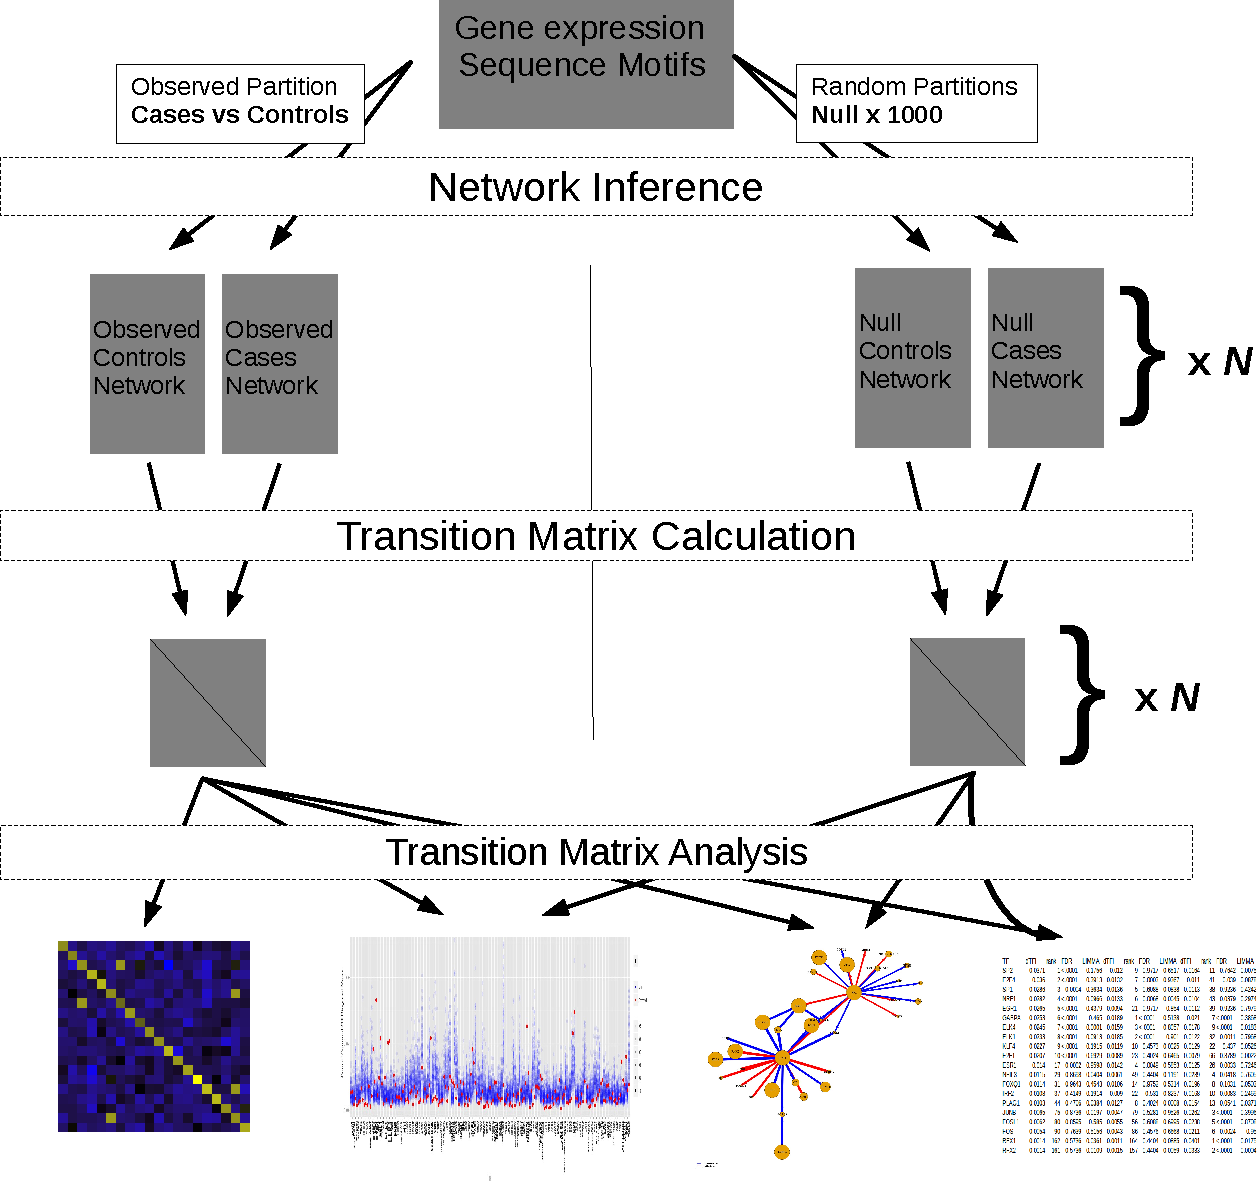
\includegraphics[width=0.8\columnwidth]{figures/workflow_diagram}\caption{\textbf{Overview of Transition Matrix analysis workflow.} (1) BERE
is applied separately to subsets of the gene expression data including
the cases group, the controls group and 1000 permutations of the cases
and controls labels. (2) Transition matrix is estimated between the
cases and controls and each of the pair or permuted ``cases'' and
``controls''.}
\end{figure}



\section*{TM significantly improves TF-TF edge estimation from simulated gene
expression data }

To evaluate the ability of our method to recover edges between transcription
factors, we generated simulated gene expression data. We began by
generating a true controls adjacency matrix, $M_{0\left(p\times q\right)}$,
describing the weighted edges between $q$ transcription factors and
$p$ genes. A state transition was generated by sampling 100 TF-TF
pairs and adjusting the edgeweight at the corresponding point on the
true cases adjacency matrix, $M_{1\left(p\times q\right)}$. These
TF-TF pairs ultimately represent the edges that we seek to recover
and the size of the adjustments are the parameters of interest. We
sampled from a multivariate Gaussian distribution with the off-diagonal
of the variance-covariance matrix, $\Sigma$, defined as the $M_{0}M_{0}^{\prime}$.
Furthermore, we scaled the magnitude of the diagonal of $\Sigma$
to achieve the desired proportion of noise. We aimed for an area under
the curve of the receiver-operator characteristic of approximately
0.70 as this has reasonably been achieved in existing biological studies~\cite{glass2013passing}.
We note that the two simulated regulatory priors have AUC-ROC of .570
and .547, which feeds the BERE and PANDA algorithms with priors which
are substantially less predictive than sequence motif priors commonly
used for network inference methods.

This sampling represented our simulated control samples. The adjusted
adjacency matrix, $M_{1}$, was similarly used to generate simulated
expression data for the cases group. Next, we reconstructed the networks
from our expression data using a set of commonly used network inference
methods - Weighted Gene Correlation Network Analysis (WGCNA)~\cite{Langfelder2008WGCNA}~\cite{Langfelder2008FastR},
Topological Overlap Measure (TOM)~\cite{ravasz2002hierarchical},
Algorithm for the Reconstruction of Gene Regulatory Networks (ARACNE)~\cite{margolin2006aracne},
Context Likelihood of Relatedness (CLR)~\cite{faith2007large}, Passing
Attributes between Networks for Data Assimilation (PANDA)~\cite{glass2013passing}
and simple Pearson correlation (PC). 

We applied the transition matrix with default parameters on each case-control
pair of networks. For comparison, we estimated the difference from
case to control in edgeweights derived from the direct edge prediction
using each network inference method. The predictions for the TM approach
and the direct approach were evaluated by the area-under-the-curve
of the receiver-operator-characteristic (AUCROC) with the true transition
adjustments taken as the gold standard. For each of the network inference
methods tested, we found substantial improvement in the predicted
transitions over the direct network inference method. In many cases,
the edgeweight difference (column 2) was not statistically significant
for predicting transitions, but when the TM was applied (column 3)
a strong predictive signal appeared. In other cases, an existing signal
was observed using the direct approach, but was dramatically improved
with the application of the TM.

The intuition behind the improvement is simple. While the estimation
of a TF-TF edge is typically evaluated via some pairwise gene expression
pattern which may be rife with technical and biological noise, the
TM approach borrows information from all downstream targets in estimating
the relative change in relationship between the TFs. 

{\tiny

\begin{table}
\begin{tabular}{|cc||c|c|}
\multicolumn{4}{c}{AUC-ROC for Edgeweight differences vs Transition Matrix using various
NI methods}\tabularnewline
\hline 
\multirow{2}{*}{\textbf{NI Method}} & \multirow{2}{*}{\textbf{Network AUC}} & \textbf{Edgeweight } & \textbf{Transition}\tabularnewline
 &  & \textbf{differences} & \textbf{Matrix}\tabularnewline
\hline 
Pearson & .704 & .510 (p=.72) & .802 (p<.0001)\tabularnewline
\hline 
WGCNA(6) & .704 & .512 (p=.61) & .688 (p<.0001)\tabularnewline
\hline 
WGCNA(12) & .704 & .52 (p=.10) & .589 (p=.02)\tabularnewline
\hline 
ARACNE & .515 & .523 (p=.58) & .566 (p=.09)\tabularnewline
\hline 
CLR & .694 & .57 (p=.19) & .814 (p<.0001)\tabularnewline
\hline 
TOM & .703 & .51 (p=.62) & .689 (p<.0001)\tabularnewline
\hline 
PANDA{*} & .747 & .520 (p=.13) & .793 (p<.0001)\tabularnewline
\hline 
PANDA{*}{*} & .652 & .509 (p=.43)  & .66 (p<.0001) \tabularnewline
\hline 
BERE{*} & .813 &  & \tabularnewline
\hline 
BERE{*}{*} & .697 &  & \tabularnewline
\hline 
\end{tabular}\caption{\textbf{Comparison of edgeweight difference to Transition Matrix in
simulated case-control gene expression}. Several network inference
methods were run on our \emph{in silico} case-control data. The overall
network area under the curve of the receiver-operator characteristic
(AUC-ROC) was performed for each method averaged across cases and
controls. For PANDA{*} and PANDA{*}{*}, which additionally utilizes
motif prior information, motif priors with AUC-ROC of .570 and .547
were used. The naive TF-TF transitions were calculated as the difference
in TF-TF edgeweight between cases and controls. The transition matrix
TF-TF transitions used the absolute transition matrix values. }
\end{table}


}


\section*{BERE: A regression-based approach to modeling gene regulatory networks }

In 2013, we described PANDA~\cite{glass2013passing}, a method~\cite{olsen2014inference}
for estimating gene regulatory networks that uses \textquotedblleft{}message
passing\textquotedblright{}�~\cite{frey2007clustering} to integrate
multiple types of genomic data. PANDA begins with a prior regulatory
network based on mapping transcription factor motifs to a reference
genome and integrates other sources of data, such as protein-protein
interaction and gene expression profiles, to estimate individual sample
networks. While PANDA has proven to be very useful in a number of
applications~\cite{lao2015genome,glass2015network,glass2014sexually},
its iterative approach to edge-weight optimization limits its utility
in situations requiring a large number of network bootstrap estimations.
To address this limitation, we developed BERE, Bipartite Edge Reconstruction
from Expression. BERE approaches the network inference problem by
considering the available evidence of an edge for each possible TF-gene
pair. This evidence can be divided into two components, referred to
here as direct and indirect. Consider the edge between a TF and a
gene, referred to here as $TF_{i}$ and $g_{j}$, respectively. The
direct evidence, $d_{i,j}$, consists of the squared conditional correlation
of the $g_{i}$ and $g_{j}$ given all other regulators of $g_{i}$.
Where $g_{i}$ is the gene which encodes $TF_{i}$ 
\[
d_{i,j}=cor\left(g_{i},g_{j}|\left\{ g_{k,-j}:k\ne j,k\in\mathbf{TF}\right\} \right)^{2}
\]
 Naturally, the use of direct evidence inadequately captures regulatory
relationships due to the impacts of technical noise and numerous biological
external factors such as stable or transient protein-protein interactions,
post-translational modifications, etc. which may confound or modify
a regulatory effect. These sources of confounding and variability
in the expression pattern of a gene coding a TF may obscure the effects
it has on all of its target genes. Therefore it is of value if we
can complement our estimate of the likelihood of a regulatory mechanism
by aggregating the information from the gene expression patterns of
all suspected targets of transcription factors. PANDA achieves its
superior performance in part by convergence towards \textquotedblleft{}agreement\textquotedblright{},
whereby large collections of gene expression patterns must agree with
the proposed regulatory structure in order to claim an interaction.
Similarly, BERE looks for agreement between the gene expression patterns
of large sets of co-targeted genes. We refer to this feature as indirect
evidence and can achieve this by again utilizing our set of regulatory
priors. In this portion of the analysis we suspend the recognition
of a TF as a member of the gene list and instead consider each of
the m TFs to be binary classifications across the entire gene list.
Class labels are determined by the presence or absence of a sequence
binding motif for that TF in the vicinity of the gene.

The indirect evidence between the two nodes, $e_{i,j}$, represents
the fitted probability that $g_{i}$ belongs to the class of genes
targeted by $TF_{j}$. $g_{i}$ is considered to be a new observation
placed into the $n-$dimensional space separated by transcription
factor targets and non-targets. To divide up the space, BERE uses
a regularized logistic regression on the gene expression data with
the training set taken to be all genes and the training labels taken
to be the existence or non-existence of a known sequence motif for
$TF_{j}$ upstream of $g_{i}$. The penalized model matrix comes from
the recognition that correlations between co-regulated genes will
be most strong when the $TF_{j}$ is most prevalent. We therefore
use the abundance of $TF_{j}$ to weight the penalized model matrix,
providing increased sensitivity for detecting coexpression for those
samples in which we most expect it to occur. To build each of our
classifiers we use the $L2$ regularization with the penalized model
matrix, $\mathbf{Q}$, a diagonal matrix with weights equal to the
the inverse expression value of the transcription factor. Effectively,
we maximize the penalized logistic likelihood function 

\[
\sum_{i=1}^{n}log\left[exp\left(\mathbf{\beta^{\prime}x_{i}}\right)^{Y_{i}}\left\{ 1-exp\left(\mathbf{\beta^{\prime}x_{i}}\right)\right\} ^{1-Y_{i}}\right]-\lambda\mathbf{\beta^{\prime}Q\beta}
\]
This computation is run using the R package \textquotedblleft{}penalized\textquotedblright{},
with the penalty term lambda estimated via default 5 fold cross validation.

By scoring each gene according to the strength of indirect evidence
for a regulatory response to each of the TFs, we can combine this
with the direct evidence of regulation (squared conditional correlation
of expression for genei and $TF_{i}$). The appropriate manner in
which to combine direct and indirect evidence remains an open question.
Though both measures are bounded by {[}0,1{]} their interpretation
is quite different. The direct evidence can be considered in terms
of it's conditional gene expression $R^{2}$ between nodes, while
the indirect evidence is interpreted as a probability. We use a non-parametric
approach to combine evidence. The targets of each TF are then ranked
and combined as a weighted sum, $w_{i}=\left(1-\alpha\right)\left[rank\left(d_{i}\right)\right]+\alpha\left[rank\left(e_{i}\right)\right]$,$i\in\left\{ 1,\dots,n\right\} $.
Our choice of the weight, $\alpha$, here is based on empirical evaluation,
and perhaps not surprisingly, is loosely correlated with organism
complexity. In validation sets from Yeast, the optimal alpha was observed
near $\alpha=.9$ while simpler E. coli datasets saw an optimal value
of $\alpha=.6$ and an in silico dataset, optimality was achieved
at $\alpha<.5$ This naturally reflects the fact that the increased
complexity of the network necessitates the use of larger scale agreement
between genes, rather than a reliance on pairwise correlations between
potentially noisier and more complex expression patterns. 


\section*{BERE recovers regulatory edges in In Silico, E. coli and Yeast (\emph{Saccharomyces
cerevisiae})}

A common challenge in gene regulatory network inference is the difficulty
of validating identified networks against a known, reliable gold standard.
A number of validation methods have been used for in vivo samples,
including ChIP-seq, ChIP-chip. Knockdowns have also been used in cell
lines and have been shown to be effective at predicting in vivo responses
\cite{olsen2014inference}. Additionally, in silico methods have been
used which simulate gene expression datasets based on a predefined
set of regulatory mechanisms.

To test our methods, we used four test datasets of increasing biological
complexity- (1) in silico, (2) E. coli, and (3) Yeast with simulated
motif priors and (4) Yeast with biological motif priors. Data from
(4) was collected from \emph{Saccharomyces cerevisiae} with TF knock-out
and stress conditions \cite{harbison2004transcriptional}. Data from
the first three sources was obtained from the publicly available DREAM5
challenge\cite{marbach2012wisdom}. This challenge asked contestants
to infer gene networks from expression data alone, using a gold standard
for evalution. Instead, we started with the gold standard and swapped
a number of edges to create the type I and type II error rates consistent
with Yeast motif priors and evaluated the performance of BERE to refine
its predictions of the true gold standard. The estimated edges in
BERE utilizing the gene expression data were demonstrated to be superior
to those of the edge prior alone.

\begin{figure}
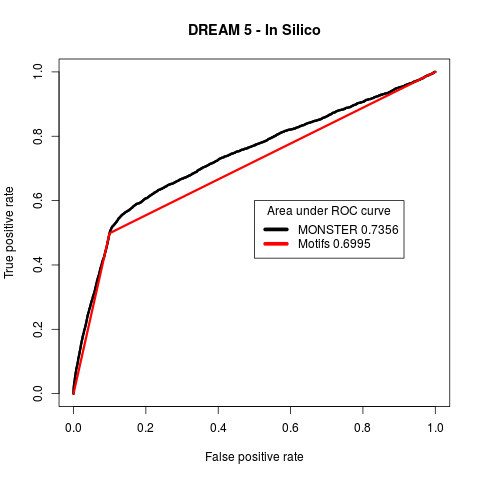
\includegraphics[width=0.4\columnwidth]{figures/DREAM5a_all}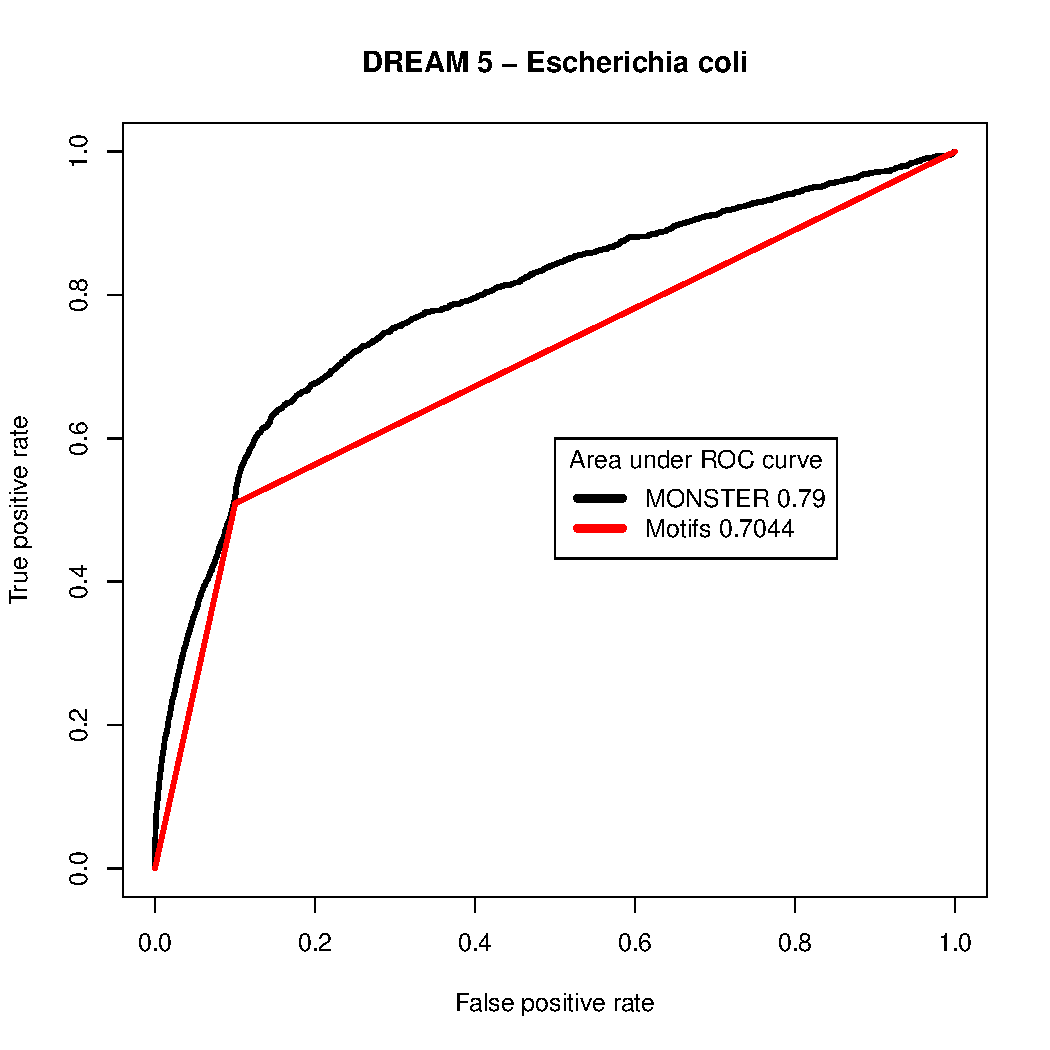
\includegraphics[width=0.4\columnwidth]{figures/DREAM5c_all}

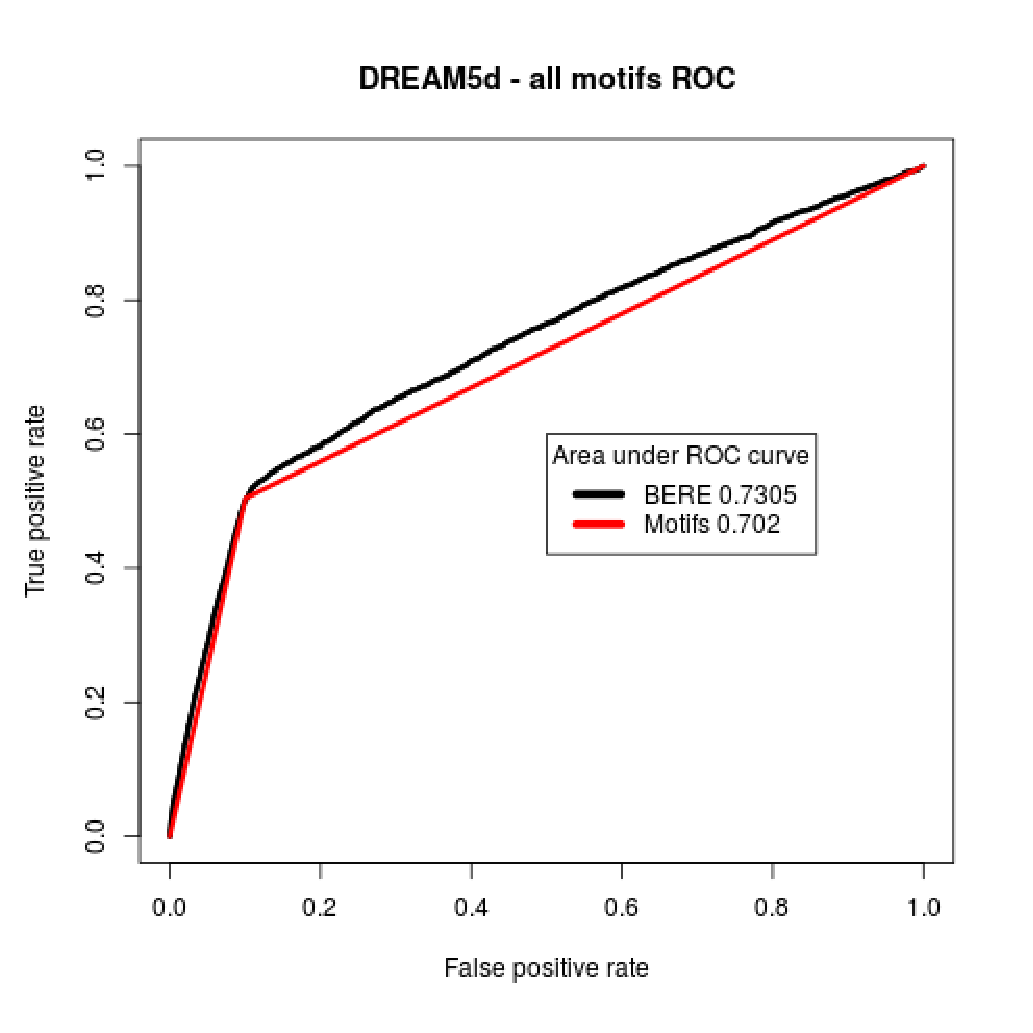
\includegraphics[width=0.4\columnwidth]{figures/DREAM5d_all}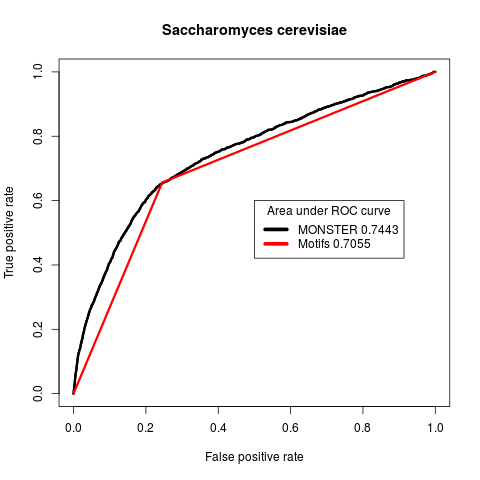
\includegraphics[width=0.4\columnwidth]{figures/Yeast_all}\caption{ROC curves for (1) in silico, (2) E. coli, (3) Yeast, demonstrating
at least comparable prediction performance for both BERE and PANDA
in refining edges beyond what is obtained using sequence motif priors.}
\end{figure}



\section*{Transition matrix finds significant protein-protein interaction}

As noted above, there are numerous biological regulatory mechanisms
which may yield detectable transitions. Of particular interest are
those which are less readily detectable via conventional methods,
such as differential gene expression analysis. One mechanism studied
here involves one TF binding to another TF to promote, suppress or
alter one or both of their regulatory patterns. These multi-protein
interactions create combinatorial complexity that can explain much
of the variation in organism complexity which is unexplained by number
of genes alone~\cite{levine2003transcription}.

To test the ability to detect protein level interactions, we compared
our estimated transitions to a set of known protein-protein interactions
\cite{ravasi2010atlas}. This set contained 223 pairwise interactions
between a total of 189 transcription factors. Of interest was the
effectiveness of identifying these interactions via the transition
from one phenotypic state to another. This is a challenging task for
several reasons, (1) protein-protein interaction is merely one of
a myraid of detectable transition mechanisms, (2) it is reasonable
to assume that only a small subset of the known PPI are actually differentially
present between case and control and (3) technological limitations
in the active field of proteomics cannot be expected to identify all
interactions with a reasonable degree of certainty.

For the transition from Smoker control to COPD, we compared for the
transition estimates to those generated by the transition from randomly
resampling the phenotypic labels. The AUCROC for the prediction of
the 223 known protein-protein interactions was $0.5695\left(p=0.018\right)$,
suggesting that our approach is successful at detecting this highly
obscured signal.
\begin{figure}[h]
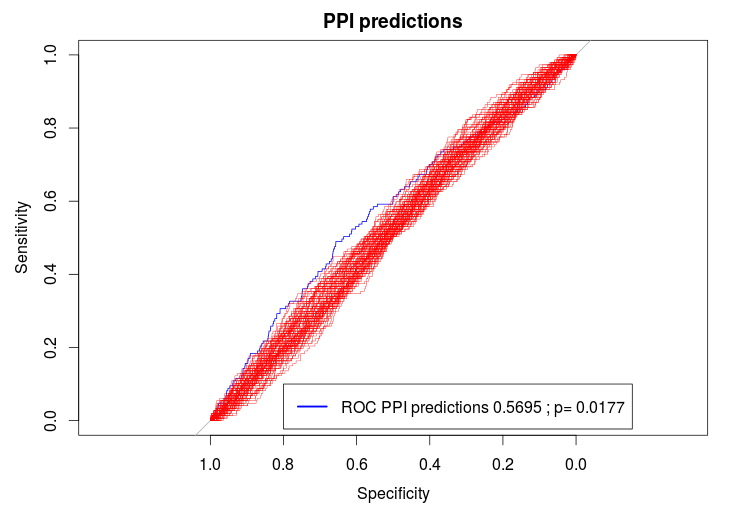
\includegraphics[width=0.5\columnwidth]{figures/pasted9a}\caption{ROC curve for prediction of PPI based on a transition from Smoker
control to COPD (blue) compared to a random case-control partition
of the ECLIPSE data.}
\end{figure}



\section*{Impact of homogeneity of cases and controls on statistical inference}

Many network inference methods use a measurement of pairwise co-expression
as a sufficient statistic for building gene networks based on gene
expression data. The ability to detect coexpression in a sample is
a function of both the level of extraneous noise and the biological
variability within the sample. In our analysis, we compared the transition
from the observed controls to observed cases and compared it to the
null distribution estimated from a randomly sampled partition of mixed
phenotypes. It is therefore of interest to consider the impact of
generating gene regulatory networks from samples with heterogeneous
versus homogeneous phenotypes. We consider whether transitions between
\emph{any} two homogeneous networks yields increased variance of test
statistics and inflation of type I error when using heterogeneous
populations for estimating the null distribution of these test statistics.

To explore, we sampled 100 cases and 100 controls. Within both cases
and controls, we split each into two groups, denoted Cases\_A, Cases\_B,
Controls\_A, Controls\_B, each of size 50. We performed BERE network
inference on each group and ran the transition matrix for each pairwise
network transition. The null networks were generated via a heterogeneous
sampling without replacement of 50 samples for the null cases and
null controls.

Of interest is the relative distribution of test statistics in transitions
across-phenotypes compared to within-phenotype, relative to the null
(heterogeneous) transitions.

We find that the distribution of dTFI for homogeneous within-phenotype
transitions (Cases\_A $\rightarrow$Cases\_B, Controls\_A $\rightarrow$
Controls\_B) closely matched the distribution of dTFI under the heterogeneous
null. Comparatively, across-phenotype transitions showed strongly
significant results compared to the heterogeneous null. We view these
results as strong evidence that our findings in this manuscript are
not inflated due to the comparison of homogeneous observed networks
relative to heterogeneous null networks.


\section*{Efficiency of estimation}

Let $\mathbf{x}_{p}$ be a Gaussian $p$-vector representing a sample
of gene expression data containing $q$ transcription factors and
$p-q$ non-transcription factor genes. 
\[
\mathbf{x}_{p}\sim N\left(\mathbf{\mu},\Sigma\right)
\]
where $\mathbf{\mu}$ is the $p$-vector of mean gene expression values
and $\Sigma$ is the $p\times p$ variance-covariance matrix. In this
scenario, $\Sigma$ may be regarded as a combination of two independent
variance-covariance sources- (1) biological signal, (2) biological
noise and technical noise.

In investigating gene regulation, many network inference methods are
constructed for the estimation of the $p\times q$ subset of $\Sigma$
pertaining to the effect of the $q$ TFs on the $p$ genes. In identifying
drivers of state transitions, we seek to focus on the $q\times q$
matrix of TF-TF effects. We show that our method vastly ourperforms
commonly used network inference methods in estimating these specific
effects.

Consider a state change between two experimental conditions, A and
B, characterized by an alteration of size $\delta$ to the biological
signal component of the TF-TF variance-covariance matrix at point
$\Sigma_{i,j}$ where $i$ and $j$ are indices for two TFs in $\Sigma$.

Using a univariate coexpression calculation (the basis for Pearson
networks and WGCNA estimates), the estimated variance of our estimate
of $\delta$ can be calculated:

\[
-\rho_{A}<\delta<\rho_{A},\delta+\rho_{A}\le1
\]


\begin{eqnarray*}
Var\left(\hat{\rho}_{i,j,A}-\hat{\rho}_{i,j,B}\right) & = & Var\left(\hat{\delta}_{cor}\right)\\
 &  & Var\left(\hat{\rho}_{i,j,A}\right)+Var\left(\hat{\rho}_{i,j,B}\right)\\
 & = & \frac{1-\rho_{i,j,A}^{2}}{n_{A}-2}+\frac{1-\rho_{i,j,B}^{2}}{n_{B}-2}\\
 & = & \frac{1}{n_{A}-2}+\frac{1}{n_{B}-2}-\frac{\rho_{i,j,A}^{2}}{n_{A}-2}-\frac{\rho_{i,j,B}^{2}}{n_{B}-2}
\end{eqnarray*}
Meanwhile, in condition B the new correlation of $TF_{i}$ with some
gene, $gene_{k}$ $k\in1,2\dots p$ , denoted $cor^{*}$, becomes
\[
cor^{*}\left(TF_{i},gene_{k}\right)=cor\left(TF_{i},gene_{k}\right)+\delta cor\left(TF_{j},gene_{k}\right)
\]
where the term $\delta cor\left(TF_{j},gene_{k}\right)$ is the change
due to the interaction of $TF_{i}$ and $TF_{j}$. 

The variance of our estimate using the transition matrix can be expressed
as follows:
\begin{eqnarray*}
Var\left(TM_{i,j}\right) & = & Var\left(\hat{\delta}_{TM}\right)\\
 & = & \frac{\left(\frac{1}{p}\right)\sum_{k=1}^{p}vVar\left(\hat{\rho}_{i,k,A}-\hat{\rho}_{i,k,B}\right)}{\sum_{k=1}^{p}\left(\rho_{j,k}-\bar{\rho_{j}}\right)^{2}}\\
\\
 & = & \frac{\left(\frac{1}{p}\right)\sum_{k=1}^{p}\left[Var\left(\hat{\rho}_{i,k,A}\right)+Var\left(\hat{\rho}_{i,k,B}\right)\right]}{\sum_{k=1}^{p}\left(\rho_{j,k}-\bar{\rho_{i}}\right)^{2}}\\
 & \le & \frac{\left(\frac{1}{p}\right)\sum_{k=1}^{p}\left[\frac{1}{n_{A}-2}+\frac{1}{n_{B}-2}\right]}{\sum_{k=1}^{p}\left(\rho_{j,k}-\bar{\rho_{i}}\right)^{2}}\\
 & \le & \frac{\frac{1}{n_{A}-2}+\frac{1}{n_{B}-2}}{\sum_{k=1}^{p}\left(\rho_{j,k}-\bar{\rho_{i}}\right)^{2}}\\
 & \le & \frac{Var\left(\hat{\delta}_{cor}\right)+\frac{\rho_{i,j,A}^{2}}{n_{A}-2}+\frac{\rho_{i,j,B}^{2}}{n_{B}-2}}{\sum_{k=1}^{p}\left(\rho_{j,k}-\bar{\rho_{i}}\right)^{2}}\\
 & \le & Var\left(\hat{\delta}_{cor}\right)+\frac{Var\left(\hat{\delta}_{cor}\right)\left(1-\sum_{k=1}^{p}\left(\rho_{j,k}-\bar{\rho_{i}}\right)^{2}\right)+\frac{\rho_{i,j,A}^{2}}{n_{A}-2}+\frac{\rho_{i,j,B}^{2}}{n_{B}-2}}{\sum_{k=1}^{p}\left(\rho_{j,k}-\bar{\rho_{i}}\right)^{2}}
\end{eqnarray*}
So we have that $Var\left(TM_{i,j}\right)<Var\left(\hat{\delta}_{cor}\right)$
when
\[
Var\left(\hat{\delta}_{cor}\right)\left(1-\sum_{k=1}^{p}\left(\rho_{j,k}-\bar{\rho_{i}}\right)^{2}\right)<\frac{\rho_{i,j,A}^{2}}{n_{A}-2}+\frac{\rho_{i,j,B}^{2}}{n_{B}-2}
\]
Since each term except $\left(1-\sum_{k=1}^{p}\left(\rho_{j,k}-\bar{\rho_{i}}\right)^{2}\right)$
is strictly non-negative, we see that this inequality holds when 
\[
\sum_{k=1}^{p}\left(\rho_{j,k}-\bar{\rho_{i}}\right)^{2}<1
\]
Thus, we have a more efficient estimator of $\delta$ when 
\[
p>\frac{1}{Var\left(\rho_{j,k}\right)}
\]
In practice, we typically have a large number of genes, $p$, so that
our transition matrix estimator will be expected to be dramatically
more efficient than the commonly used Pearson or WGCNA estimators.

\begin{table}
{\center {\tiny

\begin{tabular}{|c||c|c|c|c||c|c|c|c||c|c|c|c|}
\hline 
 & \multicolumn{4}{c||}{ECLIPSE} & \multicolumn{4}{c||}{COPDGene} & \multicolumn{4}{c|}{LGRC}\tabularnewline
\hline 
TF & dTFI & rank & FDR & LIMMA & dTFI & rank & FDR & LIMMA & dTFI & rank & FDR & LIMMA\tabularnewline
\hline 
\hline 
SP2 & .0371 &  1 & <.0001 & .1756 & .0120 &  9 & .9717 & .6517 & .0164 & 11 & .7642 & .0075\tabularnewline
\hline 
E2F4 & .0360 &  2 & <.0001 & .3913 & .0132 &  7 & .0003 & .9367 & .0110 & 41 & .039 & .0878\tabularnewline
\hline 
SP1 & .0286 &  3 & .0004 & .3634 & .0136 &  5 & .6088 & .0838 & .0113 & 38 & .9236 & .4242\tabularnewline
\hline 
NRF1 & .0282 &  4 & <.0001 & .0966 & .0133 &  6 & .0068 & .0045 & .0104 & 43 & .0379 & .2974\tabularnewline
\hline 
EGR1 & .0265 &  5 & <.0001 & .4379 & .0094 &  21 & .9717 & .8540 & .0112 & 39 & .9236 & .7979\tabularnewline
\hline 
GABPA & .0253 &  6 & <.0001 & .4650 & .0189 &  1 & <.0001 & .5138 & .0210 &  7 & <.0001 & .3868\tabularnewline
\hline 
ELK4 & .0245 &  7 & <.0001 & .0001 & .0159 &  3 & <.0001 & .8057 & .0178 &  9 & <.0001 & .0183\tabularnewline
\hline 
ELK1 & .0233 &  8 & <.0001 & .0913 & .0185 &  2 & <.0001 & .9010 & .0122 & 32 & .0011 & .7968\tabularnewline
\hline 
KLF4 & .0227 &  9 & <.0001 & .1915 & .0119 &  10 & .4573 & .0025 & .0129 & 22 & .437 & .0526\tabularnewline
\hline 
E2F1 & .0207 &  10 & <.0001 & .6929 & .0089 &  23 & .4024 & .6465 & .0079 & 66 & .3789 & .0022\tabularnewline
\hline 
ESR1 & .0140 &  17 & .0002 & .9598 & .0142 &  4 & .0049 & .5853 & .0125 & 26 & .0033 & .7246\tabularnewline
\hline 
NFIL3 & .0115 &  29 & .8698 & .0404 & .0061 &  49 & .4404 & .1191 & .0239 &  4 & .0418 & .7605\tabularnewline
\hline 
FOXQ1 & .0114 &  31 & .9643 & .4543 & .0106 &  14 & .9752 & .5314 & .0196 &  8 & .1031 & .0503\tabularnewline
\hline 
IRF2 & .0108 &  37 & .4149 & .1914 & .0090 &  22 & .531 & .8237 & .0168 & 10 & .0083 & .2469\tabularnewline
\hline 
PLAG1 & .0103 &  44 & .4706 & .0384 & .0127 &  8 & .4024 & .0008 & .0154 & 13 & .0541 & .0371\tabularnewline
\hline 
JUNB & .0065 &  75 & .8736 & .0197 & .0047 &  79 & .5281 & .9526 & .0262 &  3 & <.0001 & .3996\tabularnewline
\hline 
FOSL1 & .0062 &  80 & .8595 & .5850 & .0055 &  56 & .6088 & .6995 & .0238 &  5 & <.0001 & .8708\tabularnewline
\hline 
FOS & .0054 &  90 & .7639 & .5156 & .0043 &  86 & .4576 & .6668 & .0211 &  6 & .0024 & .9500\tabularnewline
\hline 
RFX1 & .0014 & 162 & .5736 & .0361 & .0011 & 164 & .4404 & .0885 & .0401 &  1 & <.0001 & .0175\tabularnewline
\hline 
RFX2 & .0014 & 161 & .5736 & .0109 & .0015 & 157 & .4404 & .0059 & .0333 &  2 & <.0001 & .0004\tabularnewline
\hline 
\end{tabular}}}\caption{Combined list of TFs which were among the top 10 hits (out of 166
available TFs) in any of the 3 studies, ordered by the dTFI in the
ECLIPSE study. For each study, columns indicate the TF's (1) differential
TF Involvement, (2) dTFI Rank within list of TFs, (3) Significance
of dTFI by false discovery rate, and (4) p-value for LIMMA differential
gene expression analysis.}
\end{table}


\bibliographystyle{plain}
\bibliography{dissertation_research}

\end{document}
